% chktex-file 2% chktex-file 29
% chktex-file 13
\documentclass{report}
\usepackage{setspace}
\usepackage[a4paper, total={7in, 10in}]{geometry}
\usepackage[fleqn]{amsmath}
\usepackage{empheq}
\usepackage{amssymb}
\usepackage{amsthm}
\usepackage{gensymb}
\usepackage[fleqn]{cases}
\usepackage{multicol}
\usepackage{color}
\usepackage{stix}
\usepackage{chngcntr}
\usepackage{tikz}
\usepackage{enumitem}
\usepackage{pgfplots}
\usepackage{etoolbox}
\usetikzlibrary{calc,matrix,arrows}
\usetikzlibrary{decorations.pathmorphing,patterns}

\counterwithout{equation}{chapter}
\setlength{\columnseprule}{1pt}
\setlength{\columnsep}{24pt}
\setcounter{chapter}{14}
\hfuzz=100pt

\newcommand{\pgfplotsdrawaxis}{\pgfplots@draw@axis}
\makeatother
\pgfplotsset{only axis on top/.style={axis on top=false, after end axis/.code={
                    \pgfplotsset{axis line style=opaque, ticklabel style=opaque, tick style={thick,opaque},
                        grid=none}\pgfplotsdrawaxis}}}

\newtheorem{theorem}{Theorem}

\begin{document}
\newcommand{\sol}[1]{

    \noindent \textbf{Sol.}
}
\newcommand{\prooff}[1]{

    \noindent \textbf{Proof.}
}
\newcommand\m[1]{\begin{pmatrix}#1\end{pmatrix}}
\newcommand\vm[1]{\begin{vmatrix}#1\end{vmatrix}}
\newenvironment{amatrix}[1]{%
    \left(\begin{array}{@{}*{#1}{c}|c@{}}
        }{%
    \end{array}\right)
}
\newenvironment{cequation}{
    \makeatletter
    \setbool{@fleqn}{false}
    \makeatother
    \begin{equation*}
        }{\end{equation*}}
\begin{titlepage}
    \raggedleft{}
    \rule{1pt}{\textheight}
    \hspace{0.02\textwidth}
    \parbox[b]{0.75\textwidth}{

    {\Huge\bfseries Solution Book of \\[0.5\baselineskip] Mathematic}\\[2\baselineskip]
    {\large\textit{Ssnior 2 Part I}}\\[4\baselineskip]
    {\Large\textsc{MELVIN CHIA}}

    \vspace{0.5\textheight}

    {\noindent Written on 9 October 2022}\\[\baselineskip]
    }

\end{titlepage}

\doublespacing{}
\tableofcontents
\singlespacing{}
\newpage

\begin{multicols}{2}
    \section{Linear Programming}

    \subsection{Practice 12}
    Find the maximum and minimum value of $z = 8x - 10y$ subject to the following
    constraints: \[\begin{cases}
            x + 2y \leq 40  \\
            3x + 2y \leq 90 \\
            x \geq 0        \\
            y \geq 0
        \end{cases}\]

    \subsection{Exercise 15.8}
    \begin{enumerate}
        \item Find the minimum value of $z = 10x + 12y$, subject to the following
              constraints: \[\begin{cases}
                      3x + y \geq 8   \\
                      2x + 3y \geq 15 \\
                      x + 5y \geq 9   \\
                      x \geq 0        \\
                      y \geq 0
                  \end{cases}\]
        \item A housing developer owns a tract of land that is $2,400 m^2$ in area and a
              construction capital of $\$4,600,000$. The developer wishes to build two types
              of houses: type A and type B. Given that each type A house requires $150 m^2$
              of land and $\$250,000$ of construction fees, can earn $\$55,000$ in profit;
              and each type B house requires $200 m^2$ of land and $\$400,000$ of
              construction fees, can earn $\$80,000$ in profit. Assume that all houses built
              can be sold, how many of each type of house should be built to maximize the
              profit? Find the maximum profit.

        \item One has a building lot that is $180 m^2$ in area. He plans to pay $\$7,000$ to
              split the lot into two type of rooms and rent them out to students: each bigger
              room is $20 m^2$ in area and can accommodate 5 students with a monthly rent of
              $\$225$ per student; each smaller room is $15 m^2$ in area and can accommodate
              3 students with a monthly rent of $\$250$ per student. The renovation cost for
              each bigger room is $\$700$ and for each smaller room is $\$600$. Assume that
              the source of tenants is stable, how many of each type of room should be
              divided into to maximize the profit? Find the maximum profit.

        \item Ms. Tan is a tuition teacher who teaches Mathematic subject to junior 3 and
              senior 3 students. There are a total of 5 students in each junior 3 class, each
              student pays tuition fees of $\$50$ per month, and each class is held for 4
              hours per week. There are a total of 3 students in each senior 3 class, each
              student pays tuition fees of $\$120$ per month, and each class is held for 6
              hours per week. Assume that here is a stable source of students, but the number
              of junior 3 students cannot exceed 2 times the number of senior 3 students. If
              Ms. Tan is wiling to earn at least $\$6,600$ per month, how many junior 3 and
              senior 3 classes should she held per week to minimize the number hours she has
              to teach? What's the mimimum number of hours she has to teach?

        \item A company can produce a product with two types of raw materials. The first type
              of raw material cost $\$300$, freight cost $\$50$, and can produce $90kg$ of
              the product; the second type of raw material cost $\$700$, freight cost $\$40$,
              and can produce $100kg$ of the product. If the company has a total of $\$2,100$
              to spend on raw materials and $\$200$ to spend on freight every day, what's the
              maximum amount of product that can be produced every day? How many tons of each
              type of raw material should be used?

        \item A factory uses four types of raw materials: $a$, $b$, $c$, and $d$ to produce
              two types of products: $A$ and $B$, the stock of raw materials $a$, $b$, $c$,
              and $d$ are 22, 14, 15, and 18 units respectively. Given that the required
              amount of raw materials $a$, $b$, $c$, and $d$ for producing one unit of
              product $A$ is 3, 2, 0, 3 units respectively, and the required amount of raw
              materials $a$, $b$, $c$, and $d$ for producing one unit of product $B$ is 2, 1,
              3, 0 units respectively. If each product $A$ can make a profit of $\$7,000$ and
              each product $B$ can make a profit of $\$5,000$, how many units of each product
              should be produced to maximize the profit with the current stock of raw
              materials?
        \item Mr. Wong is willing to mix two types of drinks: $A$ and $B$ to produce a new
              drink. Drink $A$ cost $\$2$ per litre, contains $20mg$ of vitamin $C$, $3mg$ of
              coloring agent, and $150g$ of sugar; drink $B$ cost $\$4$ per litre, contains
              $35mg$ of vitamin $C$, $2mg$ of coloring agent, and $100g$ of sugar. Mr. Tan is
              willing to mix at least $50$ litres of the new drink, but each litre of the new
              drink has to contain at least $30mg$ of vitamin $C$, the total amount of sugar
              cannot exceed $6kg$, and the total cost cannot exceed $\$180$. How many litres
              of each type of drink should be mixed to minimize the amount of coloring agent?

        \item A bakery bakes two types of cake: $A$ and $B$. The ingredients required for
              baking one cake of type $A$ is $1kg$ of flour, 5 eggs, and $300g$ of sugar; the
              ingredients required for baking one cake of type $B$ is $800g$ of flour, 8
              eggs, and $200g$ of sugar. The bakery has 3 bakers, each of them works for at
              least 8 hours per day, and the total time required for each baker to bake one
              cake of type $A$ and $B$ is 40 minutes and 50 minutes respectively. If the
              bakery has to bake at least 32 cakes every day, and the everyday supply of
              ingredients is limited to 220 eggs and $9kg$ of sugar. Due to the shortage of
              flour, the bakery needs to lower the usage of it. How many cakes of each type
              should be baked to minimize the usage of flour? What's the minimum amount of
              flour used?
    \end{enumerate}

    \section{Revision Exercise 15}

    Compare the algebraic expressions in the following questions (Question 1 to 2):
    \begin{enumerate}
        \item $(x-3)(4-x)$ and $(6-x)(x-1)$
              \sol{}
              \begin{flalign*}
                             & (x-3)(4-x) - (6-x)(x-1)            \\
                             & = -x^2 + 7x - 12 - (-x^2 + 7x - 6) \\
                             & = -x^2 + 7x - 12 + x^2 - 7x + 6    \\
                             & = -6 < 0                           \\
                  \therefore & \  (x-3)(4-x) < (6-x)(x-1)
              \end{flalign*}
        \item $6 - x^2$ and $4x - 2x^2$
              \sol{}
              \begin{flalign*}
                             & 6 - x^2 - (4x - 2x^2)  \\
                             & = 6x - x^2 - 4x + 2x^2 \\
                             & = x^2 - 2x             \\
                             & = {(x - 1)}^2 + 1      \\
                  \because   & \ {(x - 1)}^2 + 1 > 0  \\
                  \therefore & \ {(x - 1)}^2 + 1 > 0  \\
                  \therefore & \ 6 - x^2 > 4x - 2x^2
              \end{flalign*}
    \end{enumerate}

    \noindent Solve the following inequalities (Question 3 to 16):
    \begin{enumerate}
        \setcounter{enumi}{2}
        \item $4(x-1) > x+6$
              \sol{}
              \begin{flalign*}
                  4(x-1) & > x+6          \\
                  4x - 4 & > x+6          \\
                  3x     & > 10           \\
                  x      & > \frac{10}{3}
              \end{flalign*}
        \item $3(3-x) \geq 2(x+3)$
              \sol{}
              \begin{flalign*}
                  3(3-x) & \geq 2(x+3)      \\
                  9 - 3x & \geq 2x + 6      \\
                  -5x    & \geq -3          \\
                  5x     & \leq 3           \\
                  x      & \leq \frac{3}{5}
              \end{flalign*}
        \item $3-\frac{x-1}{4} \geq 2+\frac{3(x+1)}{8}$
              \sol{}
              \begin{flalign*}
                  3 - \frac{x-1}{4} & \geq 2 + \frac{3(x+1)}{8} \\
                  24 - 2(x-1)       & \geq 16 + 3(x+1)          \\
                  24 - 2x + 2       & \geq 16 + 3x + 3          \\
                  26 - 2x           & \geq 19 + 3x              \\
                  -5x               & \geq -7                   \\
                  5x                & \leq 7                    \\
                  x                 & \leq \frac{7}{5}
              \end{flalign*}
        \item $x-\frac{x-1}{2} \leq \frac{2x-1}{3} + \frac{x+1}{2}$
              \sol{}
              \begin{flalign*}
                  x - \frac{x-1}{2} & \leq \frac{2x-1}{3} + \frac{x+1}{2} \\
                  6x - 3(x-1)       & \leq 2(2x-1) + 3(x+1)               \\
                  6x - 3x + 3       & \leq 4x - 2 + 3x + 3                \\
                  3x + 3            & \leq 7x + 1                         \\
                  -4x               & \leq -2                             \\
                  4x                & \geq 2                              \\
                  x                 & \geq \frac{1}{2}
              \end{flalign*}
        \item $-1 < \frac{1}{2}x + 3 < 7$
              \sol{}
              \begin{flalign*}
                  -1 < \frac{1}{2}x & + 3 < 7  \\
                  -2 < x            & + 6 < 14 \\
                  -8 <              & \ x < 8
              \end{flalign*}
        \item $-\frac{3}{2} < 1 - 3x \leq 8$
              \sol{}
              \begin{flalign*}
                  -\frac{3}{2} & < 1 - 3x \leq 8      \\
                  -3           & < 2 - 6x \leq 16     \\
                  -5           & < -6x \leq 14        \\
                  -14          & \leq 6x < 5          \\
                  -\frac{7}{3} & \leq x < \frac{5}{6}
              \end{flalign*}
        \item $x^2 < 7$
              \sol{}
              \begin{flalign*}
                  x^2                      & < 7        \\
                  x^2 - 7                  & < 0        \\
                  (x+\sqrt{7})(x-\sqrt{7}) & < 0        \\
                  -\sqrt{7} < x            & < \sqrt{7}
              \end{flalign*}
              \begin{center}
                  \begin{tikzpicture}
                      \draw[latex-latex] (0,0) -- (6,0);
                      \draw[shift={(2,0)},color=black] (0pt,3pt) -- (0pt,-3pt) node[below] {$-\sqrt{7}$};
                      \draw[shift={(4,0)},color=black] (0pt,3pt) -- (0pt,-3pt) node[below] {$\sqrt{7}$};
                      \draw[shift={(1,0)},color=black] node[above] {$+$};
                      \draw[shift={(3,0)},color=black] node[above] {$-$};
                      \draw[shift={(5,0)},color=black] node[above] {$+$};
                      \node[circle,draw,fill=white,inner sep=1.5pt](a)at(2,1){};
                      \draw (a)--(4,1);
                      \node[circle,draw,fill=white,inner sep=1.5pt](b)at(4,1){};
                  \end{tikzpicture}
              \end{center}
        \item $x^2 + 10x - 200 \geq 0$
              \sol{}
              \begin{flalign*}
                  x^2 + 10x - 200               & \geq 0  \\
                  (x+20)(x-10)                  & \geq 0  \\
                  x \leq -20      \text{ or } x & \geq 10
              \end{flalign*}
              \begin{center}
                  \begin{tikzpicture}
                      \draw[latex-latex] (0,0) -- (6,0);
                      \draw[shift={(2,0)},color=black] (0pt,3pt) -- (0pt,-3pt) node[below] {$-20$};
                      \draw[shift={(4,0)},color=black] (0pt,3pt) -- (0pt,-3pt) node[below] {$10$};
                      \draw[shift={(3,0)},color=black] node[above] {$-$};
                      \draw[shift={(1,0)},color=black] node[above] {$+$};
                      \draw[shift={(5,0)},color=black] node[above] {$+$};
                      \node[circle,fill,inner sep=1.5pt](a)at(4,1){};
                      \node[circle,fill,inner sep=1.5pt](b)at(2,1){};
                      \draw[-latex,black](a)--(6,1);
                      \draw[-latex,black](b)--(0,1);
                  \end{tikzpicture}
              \end{center}
        \item $4 < 3x^2 + 4x$
              \sol{}
              \begin{flalign*}
                  4             & < 3x^2 + 4x                 \\
                  3x^2 + 4x - 4 & > 0                         \\
                  (3x-2)(x+2)   & > 0                         \\
                  x < -2        & \text{ or } x > \frac{2}{3}
              \end{flalign*}
              \begin{center}
                  \begin{tikzpicture}
                      \draw[latex-latex] (0,0) -- (6,0);
                      \draw[shift={(2,0)},color=black] (0pt,3pt) -- (0pt,-3pt) node[below] {$-2$};
                      \draw[shift={(4,0)},color=black] (0pt,3pt) -- (0pt,-3pt) node[below] {$\frac{2}{3}$};
                      \draw[shift={(1,0)},color=black] node[above] {$+$};
                      \draw[shift={(3,0)},color=black] node[above] {$-$};
                      \draw[shift={(5,0)},color=black] node[above] {$+$};
                      \node[circle,draw,fill=white,inner sep=1.5pt](a)at(2,1){};
                      \node[circle,draw,fill=white,inner sep=1.5pt](b)at(4,1){};
                      \draw[-latex,black](a)--(0,1);
                      \draw[-latex,black](b)--(6,1);
                  \end{tikzpicture}
              \end{center}
        \item $5x - 3 \geq 2x^2$
              \sol{}
              \begin{flalign*}
                  5x - 3        & \geq 2x^2        \\
                  2x^2 - 5x + 3 & \leq 0           \\
                  (2x-3)(x-1)   & \leq 0           \\
                  1 \leq x      & \leq \frac{3}{2}
              \end{flalign*}
              \begin{center}
                  \begin{tikzpicture}
                      \draw[latex-latex] (0,0) -- (6,0);
                      \draw[shift={(2,0)},color=black] (0pt,3pt) -- (0pt,-3pt) node[below] {$1$};
                      \draw[shift={(4,0)},color=black] (0pt,3pt) -- (0pt,-3pt) node[below] {$\frac{3}{2}$};
                      \draw[shift={(1,0)},color=black] node[above] {$+$};
                      \draw[shift={(3,0)},color=black] node[above] {$-$};
                      \draw[shift={(5,0)},color=black] node[above] {$+$};
                      \node[circle,fill,inner sep=1.5pt](a)at(2,1){};
                      \draw (a)--(4,1);
                      \node[circle,fill,inner sep=1.5pt](b)at(4,1){};
                  \end{tikzpicture}
              \end{center}
        \item $x^2 - x(x-6) > 5(x-1)$
              \sol{}
              \begin{flalign*}
                  x^2 - x(x-6)   & > 5(x-1) \\
                  x^2 - x^2 + 6x & > 5x - 5 \\
                  6x             & > 5x - 5 \\
                  x              & > -5
              \end{flalign*}
        \item ${(2x+1)}^2 + 5 \leq 4{(x+2)}^2$
              \sol{}
              \begin{flalign*}
                  {(2x+1)}^2 + 5    & \leq 4{(x+2)}^2      \\
                  4x^2 + 4x + 1 + 5 & \leq 4(x^2 + 4x + 4) \\
                  4x^2 + 4x + 6     & \leq 4x^2 + 16x + 16 \\
                  -12x              & \leq 10              \\
                  12x               & \geq -10             \\
                  x                 & \geq -\frac{5}{6}
              \end{flalign*}
        \item $9x^2 + 2 \leq 12x - 2$
              \sol{}
              \begin{flalign*}
                  9x^2 + 2       & \leq 12x - 2  \\
                  9x^2 - 12x + 4 & \leq 0        \\
                  {(3x - 2)}^2   & \leq 0        \\
                  x              & = \frac{2}{3}
              \end{flalign*}
        \item $4(x^2 + 7) > 3 - 20x$
              \sol{}
              \begin{flalign*}
                  4(x^2 + 7)         & > 3 - 20x             \\
                  4x^2 + 28          & > 3 - 20x             \\
                  4x^2 + 20x - 25    & > 0                   \\
                  {(2x + 5)}^2       & > 0                   \\
                  x \in \mathbb{R} , & \ x \neq -\frac{5}{2}
              \end{flalign*}
    \end{enumerate}

    \noindent Solve the following system of inequalities (Question 17 to 28):

    \begin{enumerate}
        \setcounter{enumi}{16}
        \setcounter{equation}{0}
        \item \begin{numcases}{}
                  3x + 2 \leq{0} \\
                  4-x < x
              \end{numcases}
              \sol{}
              \begin{flalign*}
                  (1):\        & 3x \leq -2          \\
                               & x \leq -\frac{2}{3} \\
                  (2):\        & -2x < -4            \\
                               & x > 2               \\
                  \\
                  \therefore\  & \text{No solution.}
              \end{flalign*}
              \begin{center}
                  \begin{tikzpicture}
                      \draw[latex-latex] (0,0) -- (6,0);
                      \draw[shift={(2,0)},color=black] (0pt,3pt) -- (0pt,-3pt) node[below] {$-\frac{2}{3}$};
                      \draw[shift={(4,0)},color=black] (0pt,3pt) -- (0pt,-3pt) node[below] {2};
                      \node[circle,fill=black,inner sep=1.5pt](a)at(2,1){};
                      \draw[-latex] (a)--(0,1);
                      \node[circle,draw,fill=white,inner sep=1.5pt](b)at(4,1){};
                      \draw[-latex] (b) -- (6, 1);
                  \end{tikzpicture}
              \end{center}

              \setcounter{equation}{0}
        \item \begin{numcases}{}
                  x + 4 > -x \\
                  \frac{3x -1}{2} < 2(x+1)
              \end{numcases}
              \sol{}
              \begin{flalign*}
                  (1):\        & 2x > -4         \\
                               & x > -2          \\
                  (2):\        & 3x - 1 < 4(x+1) \\
                               & 3x - 1 < 4x + 4 \\
                               & -x < 5          \\
                               & x > -5          \\
                  \\
                  \therefore\  & x > -2
              \end{flalign*}
              \begin{center}
                  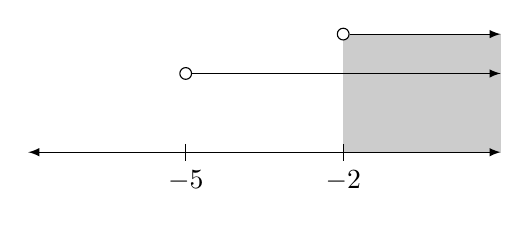
\begin{tikzpicture}
                      \fill[gray!40] (4,0) rectangle (6,1.5);
                      \draw[latex-latex] (0,0) -- (6,0);
                      \draw[shift={(2,0)},color=black] (0pt,3pt) -- (0pt,-3pt) node[below] {$-5$};
                      \draw[shift={(4,0)},color=black] (0pt,3pt) -- (0pt,-3pt) node[below] {$-2$};
                      \node[circle,draw,fill=white,inner sep=1.5pt](a)at(2,1){};
                      \draw[-latex] (a)--(6,1);
                      \node[circle,draw,fill=white,inner sep=1.5pt](b)at(4,1.5){};
                      \draw[-latex] (b) -- (6, 1.5);
                  \end{tikzpicture}
              \end{center}

              \setcounter{equation}{0}
        \item \begin{numcases}{}
                  x -3 \leq{5 -3x} \\
                  4 + (2x -1) \leq{4x + 7}
              \end{numcases}
              \sol{}
              \begin{flalign*}
                  (1):\        & 4x \leq 8          \\
                               & x \leq 2           \\
                  (2):\        & 3 + 2x \leq 4x + 7 \\
                               & -2x \leq 4         \\
                               & x \geq -2          \\
                  \\
                  \therefore\  & -2 \leq x \leq 2
              \end{flalign*}
              \begin{center}
                  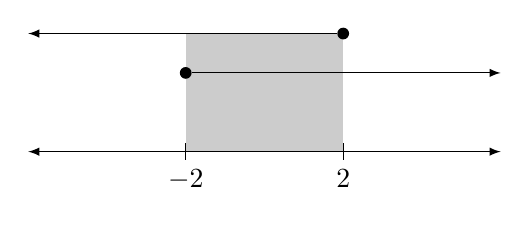
\begin{tikzpicture}
                      \fill[black!20](2,0)rectangle(4,1.5);
                      \draw[latex-latex] (0,0) -- (6,0) ;
                      \draw[shift={(2,0)},color=black] (0pt,3pt) -- (0pt,-3pt) node[below] {$-2$};
                      \draw[shift={(4,0)},color=black] (0pt,3pt) -- (0pt,-3pt) node[below] {$2$};
                      \node[circle,fill,inner sep=1.5pt](a)at(4,1.5){};
                      \node[circle,fill,inner sep=1.5pt](b)at(2,1){};
                      \draw[-latex,black](a)--(0,1.5);
                      \draw[-latex,black](b)--(6,1);
                  \end{tikzpicture}
              \end{center}

              \setcounter{equation}{0}
        \item \begin{numcases}{}
                  4x -5 \geq{2x + 1} \\
                  x + \frac{2}{3} \leq{\frac{2x + 5}{3}}
              \end{numcases}
              \sol{}
              \begin{flalign*}
                  (1): \       & 2x \geq 6          \\
                               & x \geq 3           \\
                  (2): \       & 3x + 2 \leq 2x + 5 \\
                               & x \leq 3           \\
                  \\
                  \therefore\  & x = 3
              \end{flalign*}
              \begin{center}
                  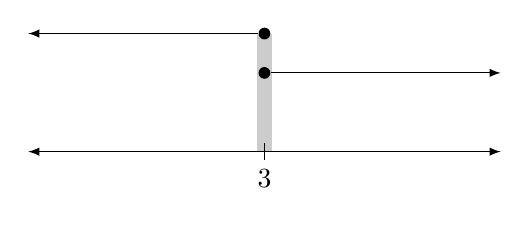
\begin{tikzpicture}
                      \fill[black!20](2.9,0)rectangle(3.1,1.5);
                      \draw[latex-latex] (0,0) -- (6,0) ;
                      \draw[shift={(3,0)},color=black] (0pt,3pt) -- (0pt,-3pt) node[below] {$3$};
                      \node[circle,fill,inner sep=1.5pt](a)at(3,1.5){};
                      \node[circle,fill,inner sep=1.5pt](b)at(3,1){};
                      \draw[-latex,black](a)--(0,1.5);
                      \draw[-latex,black](b)--(6,1);
                  \end{tikzpicture}
              \end{center}

              \setcounter{equation}{0}
        \item $5 < 2x - 7 < x + 1$
              \sol{}
              \begin{numcases}{}
                  5 < 2x -7\\
                  2x -7 < x + 1
              \end{numcases}
              \begin{flalign*}
                  (1): \       & 12 < 2x   \\
                               & x > 6     \\
                  (2): \       & x < 8     \\
                  \\
                  \therefore\  & 6 < x < 8
              \end{flalign*}
              \begin{center}
                  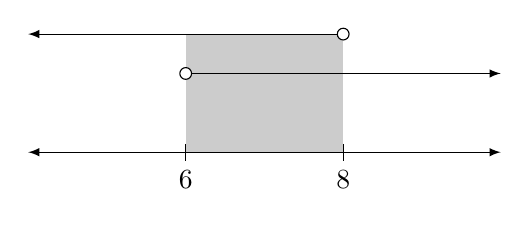
\begin{tikzpicture}
                      \fill[black!20](2,0)rectangle(4,1.5);
                      \draw[latex-latex] (0,0) -- (6,0) ;
                      \draw[shift={(2,0)},color=black] (0pt,3pt) -- (0pt,-3pt) node[below] {$6$};
                      \draw[shift={(4,0)},color=black] (0pt,3pt) -- (0pt,-3pt) node[below] {$8$};
                      \node[circle,draw,fill=white,inner sep=1.5pt](a)at(4,1.5){};
                      \node[circle,draw,fill=white,inner sep=1.5pt](b)at(2,1){};
                      \draw[-latex,black](a)--(0,1.5);
                      \draw[-latex,black](b)--(6,1);
                  \end{tikzpicture}
              \end{center}

              \setcounter{equation}{0}
        \item $4 < 6 + 2x \leq 4x$
              \sol{}
              \begin{numcases}{}
                  4 < 6 + 2x \\
                  6 + 2x \leq{4x}
              \end{numcases}
              \begin{flalign*}
                  (1): \       & -2 < 2x   \\
                               & x > -1    \\
                  (2): \       & 6 \leq 2x \\
                               & x \geq 3  \\
                  \\
                  \therefore\  & x \geq 3
              \end{flalign*}
              \begin{center}
                  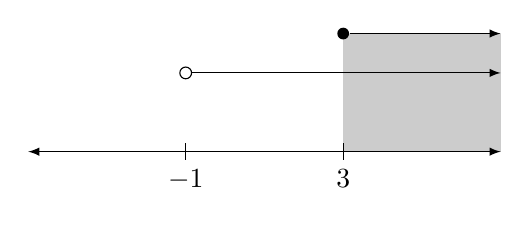
\begin{tikzpicture}
                      \fill[gray!40] (4,0) rectangle (6,1.5);
                      \draw[latex-latex] (0,0) -- (6,0);
                      \draw[shift={(2,0)},color=black] (0pt,3pt) -- (0pt,-3pt) node[below] {$-1$};
                      \draw[shift={(4,0)},color=black] (0pt,3pt) -- (0pt,-3pt) node[below] {$3$};
                      \node[circle,draw,fill=white,inner sep=1.5pt](a)at(2,1){};
                      \draw[-latex] (a)--(6,1);
                      \node[circle,fill,inner sep=1.5pt](b)at(4,1.5){};
                      \draw[-latex] (b) -- (6, 1.5);
                  \end{tikzpicture}
              \end{center}

              \setcounter{equation}{0}
        \item \begin{numcases}{}
                  x -\frac{1}{2} \geq{1 -\frac{x}{2}} \\
                  2 -\frac{x}{3} < \frac{2x}{3} -3    \\
                  \frac{x}{3} + \frac{1}{4} \geq{\frac{x}{2} -\frac{3}{4}}
              \end{numcases}
              \sol{}
              \begin{flalign*}
                  (1): \       & 2x - 1 \geq 2 - x  \\
                               & 3x \geq 3          \\
                               & x \geq 1           \\
                  (2): \       & 6 - x < 2x - 9     \\
                               & -3x < -15          \\
                               & x > 5              \\
                  (3): \       & 4x + 3 \geq 6x - 9 \\
                               & -2x \geq -12       \\
                               & x \leq 6           \\
                  \\
                  \therefore\  & 5 < x \leq 6
              \end{flalign*}
              \begin{center}
                  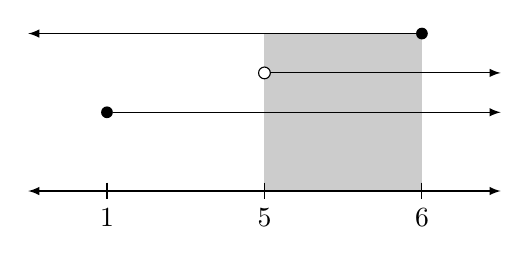
\begin{tikzpicture}
                      \fill[gray!40] (3,0) rectangle (5,2);
                      \draw[latex-latex] (0,0) -- (6,0);
                      \draw[shift={(1,0)},color=black] (0pt,3pt) -- (0pt,-3pt) node[below] {$1$};
                      \draw[shift={(3,0)},color=black] (0pt,3pt) -- (0pt,-3pt) node[below] {$5$};
                      \draw[shift={(5,0)},color=black] (0pt,3pt) -- (0pt,-3pt) node[below] {$6$};
                      \node[circle,fill,inner sep=1.5pt](a)at(1,1){};
                      \draw[-latex] (a)--(6,1);
                      \node[circle,draw,fill=white,inner sep=1.5pt](b)at(3 ,1.5){};
                      \draw[-latex] (b) -- (6, 1.5);
                      \node[circle,fill,inner sep=1.5pt](b)at(5 ,2){};
                      \draw[-latex] (b) -- (0, 2);
                  \end{tikzpicture}
              \end{center}

              \setcounter{equation}{0}
        \item \begin{numcases}{}
                  x + \frac{13}{2} > \frac{7 -x}{2}  \\
                  2\left(x+\frac{1}{3}\right) < 2 -x \\
                  x^2 \geq{\frac{5x}{2}}
              \end{numcases}
              \sol{}
              \begin{flalign*}
                  (1): \        & 2x + 13 > 7 - x                                                                                                    \\
                                & 3x > -6                                                                                                            \\
                                & x > -2                                                                                                             \\
                  (2): \        & 2x + \frac{2}{3} < 2 - x                                                                                           \\
                                & 6x + 2 < 6 - 3x                                                                                                    \\
                                & 9x < 4                                                                                                             \\
                                & x < \frac{4}{9}                                                                                                    \\
                  (3): \        & 2x^2 \geq 5x                                                                                                       \\
                                & 2x^2 - 5x \geq 0                                                                                                   \\
                                & x(2x - 5) \geq 0                                                                                                   \\
                                & x \leq 0 \text{ or } x \geq \frac{5}{2}
                                & 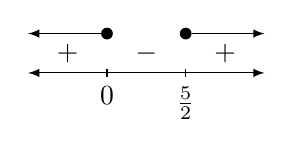
\begin{tikzpicture}[baseline={(current bounding box.center)},scale=0.5]
                                      \draw[latex-latex] (0,0) -- (6,0);
                                      \draw[shift={(2,0)},color=black] (0pt,3pt) -- (0pt,-3pt) node[below] {$0$};
                                      \draw[shift={(4,0)},color=black] (0pt,3pt) -- (0pt,-3pt) node[below] {$\frac{5}{2}$};
                                      \draw[shift={(1,0)},color=black] node[above] {$+$};
                                      \draw[shift={(3,0)},color=black] node[above] {$-$};
                                      \draw[shift={(5,0)},color=black] node[above] {$+$};
                                      \node[circle,fill,inner sep=1.5pt](a)at(2,1){};
                                      \draw[-latex](a)--(0,1);
                                      \node[circle,fill,inner sep=1.5pt](b)at(4,1){};
                                      \draw[-latex](b)--(6,1);
                                  \end{tikzpicture} \\
                  \therefore \  & -2 < x \leq 0
              \end{flalign*}
              \begin{center}
                  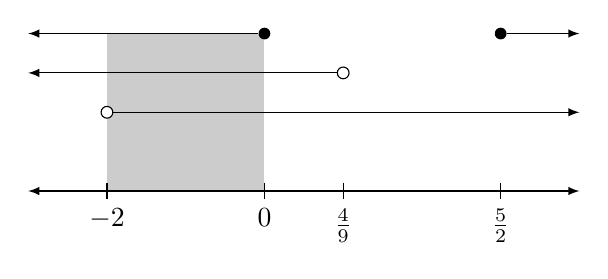
\begin{tikzpicture}
                      \fill[gray!40] (3,0) rectangle (1,2);
                      \draw[latex-latex] (0,0) -- (7,0);
                      \draw[shift={(1,0)},color=black] (0pt,3pt) -- (0pt,-3pt) node[below] {$-2$};
                      \draw[shift={(3,0)},color=black] (0pt,3pt) -- (0pt,-3pt) node[below] {$0$};
                      \draw[shift={(4,0)},color=black] (0pt,3pt) -- (0pt,-3pt) node[below] {$\frac{4}{9}$};
                      \draw[shift={(6,0)},color=black] (0pt,3pt) -- (0pt,-3pt) node[below] {$\frac{5}{2}$};
                      \node[circle,draw,fill=white,inner sep=1.5pt](a)at(1,1){};
                      \draw[-latex] (a)--(7,1);
                      \node[circle,draw,fill=white,inner sep=1.5pt](b)at(4 ,1.5){};
                      \draw[-latex] (b) -- (0, 1.5);
                      \node[circle,fill,inner sep=1.5pt](b)at(3,2){};
                      \draw[-latex] (b) -- (0, 2);
                      \node[circle,fill,inner sep=1.5pt](b)at(6,2){};
                      \draw[-latex] (b) -- (7, 2);
                  \end{tikzpicture}
              \end{center}

              \setcounter{equation}{0}
        \item \begin{numcases}{}
                  x^2 -3x -4 \geq{0} \\
                  2x^2 -x -6 > 0
              \end{numcases}
              \sol{}
              \begin{flalign*}
                  (1): \       & (x-4)(x+1) \geq 0                                                                                                   \\
                               & x \leq -1 \text{ or } x \geq 4
                               & 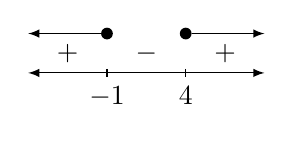
\begin{tikzpicture}[baseline={(current bounding box.center)},scale=0.5]
                                     \draw[latex-latex] (0,0) -- (6,0);
                                     \draw[shift={(2,0)},color=black] (0pt,3pt) -- (0pt,-3pt) node[below] {$-1$};
                                     \draw[shift={(4,0)},color=black] (0pt,3pt) -- (0pt,-3pt) node[below] {$4$};
                                     \draw[shift={(1,0)},color=black] node[above] {$+$};
                                     \draw[shift={(3,0)},color=black] node[above] {$-$};
                                     \draw[shift={(5,0)},color=black] node[above] {$+$};
                                     \node[circle,fill,inner sep=1.5pt](a)at(2,1){};
                                     \draw[-latex](a)--(0,1);
                                     \node[circle,fill,inner sep=1.5pt](b)at(4,1){};
                                     \draw[-latex](b)--(6,1);
                                 \end{tikzpicture}                       \\
                  (2): \       & (2x+3)(x-2) > 0                                                                                                     \\
                               & x < -\frac{3}{2} \text{ and } x > 2
                               & 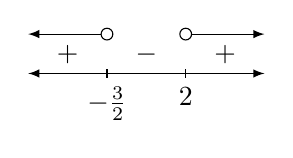
\begin{tikzpicture}[baseline={(current bounding box.center)},scale=0.5]
                                     \draw[latex-latex] (0,0) -- (6,0);
                                     \draw[shift={(2,0)},color=black] (0pt,3pt) -- (0pt,-3pt) node[below] {$-\frac{3}{2}$};
                                     \draw[shift={(4,0)},color=black] (0pt,3pt) -- (0pt,-3pt) node[below] {$2$};
                                     \draw[shift={(1,0)},color=black] node[above] {$+$};
                                     \draw[shift={(3,0)},color=black] node[above] {$-$};
                                     \draw[shift={(5,0)},color=black] node[above] {$+$};
                                     \node[circle,draw,fill=white,inner sep=1.5pt](a)at(2,1){};
                                     \draw[-latex](a)--(0,1);
                                     \node[circle,draw,fill=white,inner sep=1.5pt](b)at(4,1){};
                                     \draw[-latex](b)--(6,1);
                                 \end{tikzpicture}
                  \\
                  \\
                  \therefore\  & x < -\frac{3}{2} \text{ or } x \geq 4
              \end{flalign*}
              \begin{center}
                  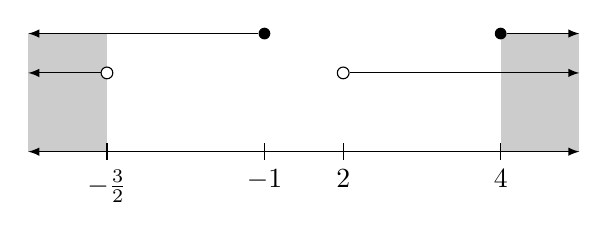
\begin{tikzpicture}
                      \fill[gray!40] (1,0) rectangle (0,1.5);
                      \fill[gray!40] (6,0) rectangle (7,1.5);
                      \draw[latex-latex] (0,0) -- (7,0);
                      \draw[shift={(1,0)},color=black] (0pt,3pt) -- (0pt,-3pt) node[below] {$-\frac{3}{2}$};
                      \draw[shift={(3,0)},color=black] (0pt,3pt) -- (0pt,-3pt) node[below] {$-1$};
                      \draw[shift={(4,0)},color=black] (0pt,3pt) -- (0pt,-3pt) node[below] {$2$};
                      \draw[shift={(6,0)},color=black] (0pt,3pt) -- (0pt,-3pt) node[below] {$4$};
                      \node[circle,draw,fill=white,inner sep=1.5pt](a)at(1,1){};
                      \draw[-latex] (a)--(0,1);
                      \node[circle,draw,fill=white,inner sep=1.5pt](b)at(4 ,1){};
                      \draw[-latex] (b) -- (7, 1);
                      \node[circle,fill,inner sep=1.5pt](c)at(3, 1.5){};
                      \draw[-latex] (c) -- (0, 1.5);
                      \node[circle,fill,inner sep=1.5pt](d)at(6,1.5){};
                      \draw[-latex] (d) -- (7, 1.5);
                  \end{tikzpicture}
              \end{center}

              \setcounter{equation}{0}
        \item \begin{numcases}{}
                  (2x -1) (x-2) \leq{8x -9} \\
                  3(x^2 -2) < 7x
              \end{numcases}
              \sol{}
              \begin{flalign*}
                  (1): \       & 2x^2 - 5x + 2 \leq 8x - 9                                                                                           \\
                               & 2x^2 - 13x + 11 \leq 0                                                                                              \\
                               & (2x - 11)(x - 1) \leq 0                                                                                             \\
                               & 1 \leq x \leq \frac{11}{2}
                               & 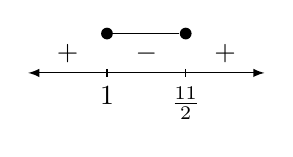
\begin{tikzpicture}[baseline={(current bounding box.center)},scale=0.5]
                                     \draw[latex-latex] (0,0) -- (6,0);
                                     \draw[shift={(2,0)},color=black] (0pt,3pt) -- (0pt,-3pt) node[below] {$1$};
                                     \draw[shift={(4,0)},color=black] (0pt,3pt) -- (0pt,-3pt) node[below] {$\frac{11}{2}$};
                                     \draw[shift={(1,0)},color=black] node[above] {$+$};
                                     \draw[shift={(3,0)},color=black] node[above] {$-$};
                                     \draw[shift={(5,0)},color=black] node[above] {$+$};
                                     \node[circle,fill,inner sep=1.5pt](a)at(2,1){};
                                     \node[circle,fill,inner sep=1.5pt](b)at(4,1){};
                                     \draw(b)--(a);
                                 \end{tikzpicture}  \\
                  (2): \       & 3x^2 - 6 < 7x                                                                                                       \\
                               & 3x^2 - 7x - 6 < 0                                                                                                   \\
                               & (3x + 2)(x - 3) < 0                                                                                                 \\
                               & -\frac{2}{3} < x < 3
                               & 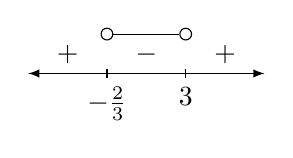
\begin{tikzpicture}[baseline={(current bounding box.center)},scale=0.5]
                                     \draw[latex-latex] (0,0) -- (6,0);
                                     \draw[shift={(2,0)},color=black] (0pt,3pt) -- (0pt,-3pt) node[below] {$-\frac{2}{3}$};
                                     \draw[shift={(4,0)},color=black] (0pt,3pt) -- (0pt,-3pt) node[below] {$3$};
                                     \draw[shift={(1,0)},color=black] node[above] {$+$};
                                     \draw[shift={(3,0)},color=black] node[above] {$-$};
                                     \draw[shift={(5,0)},color=black] node[above] {$+$};
                                     \node[circle,draw,fill=white,inner sep=1.5pt](a)at(2,1){};
                                     \node[circle,draw,fill=white,inner sep=1.5pt](b)at(4,1){};
                                     \draw(b)--(a);
                                 \end{tikzpicture} \\
                  \\
                  \therefore\  & 1 \leq x < 3
              \end{flalign*}
              \begin{center}
                  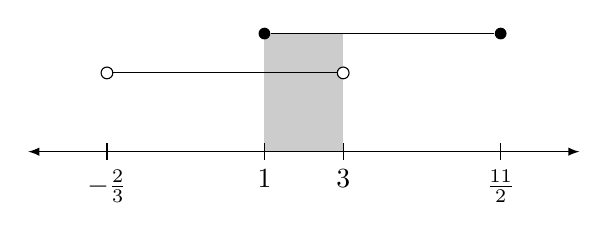
\begin{tikzpicture}
                      \fill[gray!40] (3,0) rectangle (4,1.5);
                      \draw[latex-latex] (0,0) -- (7,0);
                      \draw[shift={(1,0)},color=black] (0pt,3pt) -- (0pt,-3pt) node[below] {$-\frac{2}{3}$};
                      \draw[shift={(3,0)},color=black] (0pt,3pt) -- (0pt,-3pt) node[below] {$1$};
                      \draw[shift={(4,0)},color=black] (0pt,3pt) -- (0pt,-3pt) node[below] {$3$};
                      \draw[shift={(6,0)},color=black] (0pt,3pt) -- (0pt,-3pt) node[below] {$\frac{11}{2}$};
                      \node[circle,draw,fill=white,inner sep=1.5pt](a)at(1,1){};
                      \node[circle,draw,fill=white,inner sep=1.5pt](b)at(4 ,1){};
                      \draw (b) -- (a);
                      \node[circle,fill,inner sep=1.5pt](c)at(3, 1.5){};
                      \node[circle,fill,inner sep=1.5pt](d)at(6,1.5){};
                      \draw (d) -- (c);
                  \end{tikzpicture}
              \end{center}

              \setcounter{equation}{0}
        \item \begin{numcases}{}
                  2(x^2 + 3) \geq{7 -x} \\
                  {(x+3)}^2 > 1
              \end{numcases}
              \sol{}
              \begin{flalign*}
                  (1): \                                                                                                              & 2x^2 + 6 \geq 7 - x                                              & \\
                                                                                                                                      & 2x^2 + x - 1 \geq 0                                              & \\
                                                                                                                                      & (2x - 1)(x + 1) \geq 0                                           & \\
                                                                                                                                      & x \leq -1 \text{ or } x \geq \frac{1}{2}\ \ \ \ \ \ \ \ \
                  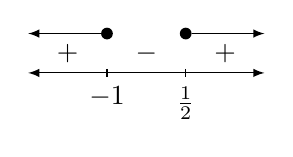
\begin{tikzpicture}[baseline={(current bounding box.center)},scale=0.5]
                      \draw[latex-latex] (0,0) -- (6,0);
                      \draw[shift={(2,0)},color=black] (0pt,3pt) -- (0pt,-3pt) node[below] {$-1$};
                      \draw[shift={(4,0)},color=black] (0pt,3pt) -- (0pt,-3pt) node[below] {$\frac{1}{2}$};
                      \draw[shift={(1,0)},color=black] node[above] {$+$};
                      \draw[shift={(3,0)},color=black] node[above] {$-$};
                      \draw[shift={(5,0)},color=black] node[above] {$+$};
                      \node[circle,fill,inner sep=1.5pt](a)at(2,1){};
                      \draw[-latex](a)--(0,1);
                      \node[circle,fill,inner sep=1.5pt](b)at(4,1){};
                      \draw[-latex](b)--(6,1);
                  \end{tikzpicture} &
                  \\
                  (2): \                                                                                                              & x^2 + 6x + 9 > 1                                                 & \\
                                                                                                                                      & x^2 + 6x + 8 > 0                                                 & \\
                                                                                                                                      & (x + 4)(x + 2) > 0                                               & \\
                                                                                                                                      & x < -4 \text{ or } x > -2\ \ \ \ \ \ \ \ \
                  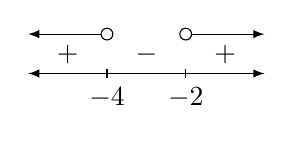
\begin{tikzpicture}[baseline={(current bounding box.center)},scale=0.5]
                      \draw[latex-latex] (0,0) -- (6,0);
                      \draw[shift={(2,0)},color=black] (0pt,3pt) -- (0pt,-3pt) node[below] {$-4$};
                      \draw[shift={(4,0)},color=black] (0pt,3pt) -- (0pt,-3pt) node[below] {$-2$};
                      \draw[shift={(1,0)},color=black] node[above] {$+$};
                      \draw[shift={(3,0)},color=black] node[above] {$-$};
                      \draw[shift={(5,0)},color=black] node[above] {$+$};
                      \node[circle,draw,fill=white,inner sep=1.5pt](a)at(2,1){};
                      \draw[-latex](a)--(0,1);
                      \node[circle,draw,fill=white,inner sep=1.5pt](b)at(4,1){};
                      \draw[-latex](b)--(6,1);
                  \end{tikzpicture}                      &
                  \\
                  \\
                  \therefore\                                                                                                         & x < -4 \text{ or } -2 < x \leq -1 \text{ or } x \geq \frac{1}{2}
              \end{flalign*}
              \begin{center}
                  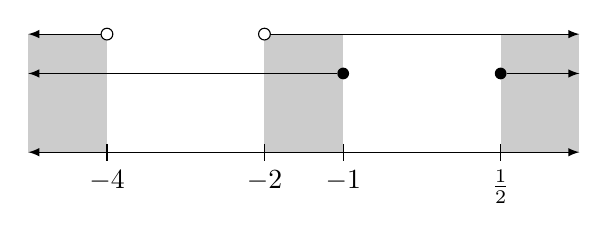
\begin{tikzpicture}
                      \fill[gray!40] (1,0) rectangle (0,1.5);
                      \fill[gray!40] (6,0) rectangle (7,1.5);
                      \fill[gray!40] (3,0) rectangle (4,1.5);
                      \draw[latex-latex] (0,0) -- (7,0);
                      \draw[shift={(1,0)},color=black] (0pt,3pt) -- (0pt,-3pt) node[below] {$-4$};
                      \draw[shift={(3,0)},color=black] (0pt,3pt) -- (0pt,-3pt) node[below] {$-2$};
                      \draw[shift={(4,0)},color=black] (0pt,3pt) -- (0pt,-3pt) node[below] {$-1$};
                      \draw[shift={(6,0)},color=black] (0pt,3pt) -- (0pt,-3pt) node[below] {$\frac{1}{2}$};
                      \node[circle,fill,inner sep=1.5pt](a)at(4,1){};
                      \draw[-latex] (a)--(0,1);
                      \node[circle,fill,inner sep=1.5pt](b)at(6 ,1){};
                      \draw[-latex] (b) -- (7, 1);
                      \node[circle,draw,fill=white,inner sep=1.5pt](c)at(1, 1.5){};
                      \draw[-latex] (c) -- (0, 1.5);
                      \node[circle,draw,fill=white,inner sep=1.5pt](d)at(3,1.5){};
                      \draw[-latex] (d) -- (7, 1.5);
                  \end{tikzpicture}
              \end{center}

              \setcounter{equation}{0}
        \item \begin{numcases}{}
                  x (x-1) \leq{2} \\
                  x (x+1) \geq{6}
              \end{numcases}
              \sol{}
              \begin{flalign*}
                  (1): \       & x^2 - x \leq 2                                                                                 \\
                               & x^2 - x - 2 \leq 0                                                                             \\
                               & (x - 2)(x + 1) \leq 0                                                                          \\
                               & -1 \leq x \leq 2
                               & 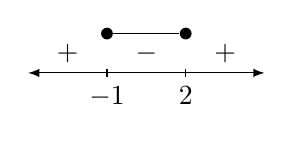
\begin{tikzpicture}[baseline={(current bounding box.center)},scale=0.5]
                                     \draw[latex-latex] (0,0) -- (6,0);
                                     \draw[shift={(2,0)},color=black] (0pt,3pt) -- (0pt,-3pt) node[below] {$-1$};
                                     \draw[shift={(4,0)},color=black] (0pt,3pt) -- (0pt,-3pt) node[below] {$2$};
                                     \draw[shift={(1,0)},color=black] node[above] {$+$};
                                     \draw[shift={(3,0)},color=black] node[above] {$-$};
                                     \draw[shift={(5,0)},color=black] node[above] {$+$};
                                     \node[circle,fill,inner sep=1.5pt](a)at(2,1){};
                                     \node[circle,fill,inner sep=1.5pt](b)at(4,1){};
                                     \draw(b)--(a);
                                 \end{tikzpicture}  \\
                  (2): \       & x^2 + x \geq 6                                                                                 \\
                               & x^2 + x - 6 \geq 0                                                                             \\
                               & (x + 3)(x - 2) \geq 0                                                                          \\
                               & x \leq -3 \text{ or } x \geq 2
                               & 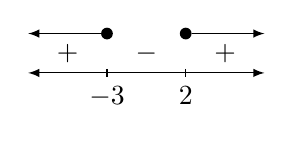
\begin{tikzpicture}[baseline={(current bounding box.center)},scale=0.5]
                                     \draw[latex-latex] (0,0) -- (6,0);
                                     \draw[shift={(2,0)},color=black] (0pt,3pt) -- (0pt,-3pt) node[below] {$-3$};
                                     \draw[shift={(4,0)},color=black] (0pt,3pt) -- (0pt,-3pt) node[below] {$2$};
                                     \draw[shift={(1,0)},color=black] node[above] {$+$};
                                     \draw[shift={(3,0)},color=black] node[above] {$-$};
                                     \draw[shift={(5,0)},color=black] node[above] {$+$};
                                     \node[circle,fill,inner sep=1.5pt](a)at(2,1){};
                                     \node[circle,fill,inner sep=1.5pt](b)at(4,1){};
                                     \draw[-latex] (b)--(6,1);
                                     \draw[-latex] (a)--(0,1);
                                 \end{tikzpicture} \\
                  \\
                  \therefore\  & x = 2
              \end{flalign*}
              \begin{center}
                  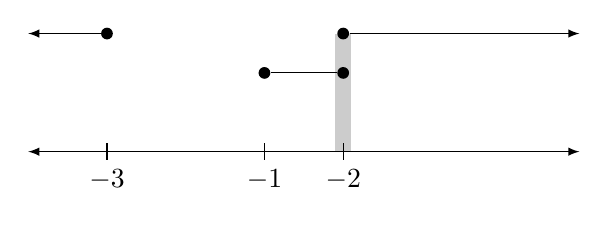
\begin{tikzpicture}
                      \fill[gray!40] (3.9,0) rectangle (4.1,1.5);
                      \draw[latex-latex] (0,0) -- (7,0);
                      \draw[shift={(1,0)},color=black] (0pt,3pt) -- (0pt,-3pt) node[below] {$-3$};
                      \draw[shift={(3,0)},color=black] (0pt,3pt) -- (0pt,-3pt) node[below] {$-1$};
                      \draw[shift={(4,0)},color=black] (0pt,3pt) -- (0pt,-3pt) node[below] {$-2$};
                      \node[circle,fill,inner sep=1.5pt](a)at(3,1){};
                      \node[circle,fill,inner sep=1.5pt](b)at(4 ,1){};
                      \draw (b) -- (a);
                      \node[circle,fill,inner sep=1.5pt](c)at(1, 1.5){};
                      \draw[-latex] (c) -- (0, 1.5);
                      \node[circle,fill,inner sep=1.5pt](d)at(4,1.5){};
                      \draw[-latex] (d) -- (7, 1.5);
                  \end{tikzpicture}
              \end{center}
    \end{enumerate}

    \noindent Solve the following inequalities (Question 29 to 40):

    \begin{enumerate}
        \setcounter{enumi}{28}
        \item $x^4 - 5x^2 + 4 \leq 0$
              \sol{}
              \begin{flalign*}
                  x^4 - 5x^2 + 4                         & \leq 0 \\
                  (x-1)(x^3 + x^2 - 4x - 4)              & \leq 0 \\
                  (x-1)(x+1)(x^2 - 4)                    & \leq 0 \\
                  (x-1)(x+1)(x-2)(x+2)                   & \leq 0 \\
                  -2 \leq x \leq -1 \text{ or } 1 \leq x & \leq 2
              \end{flalign*}
              \begin{center}
                  \begin{tikzpicture}
                      \draw[latex-latex] (0,0) -- (7,0);
                      \draw[shift={(1,0)},color=black] (0pt,3pt) -- (0pt,-3pt) node[below] {$-2$};
                      \draw[shift={(2.5,0)},color=black] (0pt,3pt) -- (0pt,-3pt) node[below] {$-1$};
                      \draw[shift={(4.5,0)},color=black] (0pt,3pt) -- (0pt,-3pt) node[below] {$1$};
                      \draw[shift={(6,0)},color=black] (0pt,3pt) -- (0pt,-3pt) node[below] {$2$};
                      \draw[shift={(0.5,0)},color=black] node[above] {$+$};
                      \draw[shift={(1.75,0)},color=black] node[above] {$-$};
                      \draw[shift={(3.5,0)},color=black] node[above] {$+$};
                      \draw[shift={(5.25,0)},color=black] node[above] {$-$};
                      \draw[shift={(6.5,0)},color=black] node[above] {$+$};
                      \node[circle,fill,inner sep=1.5pt](a)at(4.5,1){};
                      \node[circle,fill,inner sep=1.5pt](b)at(6,1){};
                      \draw (a)--(b);
                      \node[circle,fill,inner sep=1.5pt](c)at(1,1){};
                      \node[circle,fill,inner sep=1.5pt](d)at(2.5,1){};
                      \draw (c)--(d);
                  \end{tikzpicture}
              \end{center}
        \item $(x^2 + 2x - 8)(x^2 + 2x - 3) > 0$
              \sol{}
              \begin{flalign*}
                  (x+4)(x-2)(x+3)(x-1)                         & > 0 \\
                  x < -4 \text{ or } -3 < x < -1 \text{ or } x & > 2
              \end{flalign*}
              \begin{center}
                  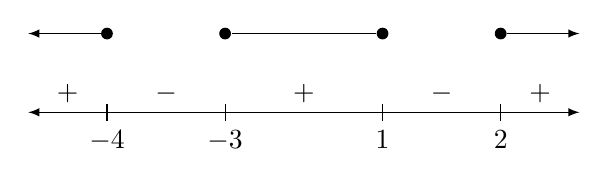
\begin{tikzpicture}
                      \draw[latex-latex] (0,0) -- (7,0);
                      \draw[shift={(1,0)},color=black] (0pt,3pt) -- (0pt,-3pt) node[below] {$-4$};
                      \draw[shift={(2.5,0)},color=black] (0pt,3pt) -- (0pt,-3pt) node[below] {$-3$};
                      \draw[shift={(4.5,0)},color=black] (0pt,3pt) -- (0pt,-3pt) node[below] {$1$};
                      \draw[shift={(6,0)},color=black] (0pt,3pt) -- (0pt,-3pt) node[below] {$2$};
                      \draw[shift={(0.5,0)},color=black] node[above] {$+$};
                      \draw[shift={(1.75,0)},color=black] node[above] {$-$};
                      \draw[shift={(3.5,0)},color=black] node[above] {$+$};
                      \draw[shift={(5.25,0)},color=black] node[above] {$-$};
                      \draw[shift={(6.5,0)},color=black] node[above] {$+$};
                      \node[circle,fill,inner sep=1.5pt](a)at(4.5,1){};
                      \node[circle,fill,inner sep=1.5pt](b)at(6,1){};
                      \node[circle,fill,inner sep=1.5pt](c)at(1,1){};
                      \node[circle,fill,inner sep=1.5pt](d)at(2.5,1){};
                      \draw [-latex] (b) -- (7, 1);
                      \draw (a)--(d);
                      \draw [-latex] (c) -- (0, 1);
                  \end{tikzpicture}
              \end{center}

        \item ${(2x + 1)}^2(x^2 + 3x - 10) < 0$
              \sol{}
              \begin{flalign*}
                  \text{For all real numbers }x                          & ,                 \\
                  {(2x+1)}^2                     > 0 \text{ when } x     & \neq -\frac{1}{2} \\
                  x^2 + 3x - 10                                          & < 0               \\
                  (x+5)(x-2)                                             & < 0               \\
                  \therefore\ -5 < x                                     & < -2              \\
                  \text{When } x = -\frac{1}{2}                          & ,                 \\
                  {(2x + 1)}^2(x^2 + 3x - 10)                            & = 0               \\
                  \therefore\ x = -\frac{1}{2} \text{ is not a }         & \text{solution.}  \\
                  \\
                  \therefore\ -5 < x < -2                           ,\ x & \neq -\frac{1}{2}
              \end{flalign*}
              \begin{center}
                  \begin{tikzpicture}
                      \draw[latex-latex] (0,0) -- (6,0);
                      \draw[shift={(2,0)},color=black] (0pt,3pt) -- (0pt,-3pt) node[below] {$-5$};
                      \draw[shift={(4,0)},color=black] (0pt,3pt) -- (0pt,-3pt) node[below] {$-2$};
                      \draw[shift={(1,0)},color=black] node[above] {$+$};
                      \draw[shift={(3,0)},color=black] node[above] {$-$};
                      \draw[shift={(5,0)},color=black] node[above] {$+$};
                      \node[circle,draw,fill=white,inner sep=1.5pt](a)at(2,1){};
                      \draw (a)--(4,1);
                      \node[circle,draw,fill=white,inner sep=1.5pt](b)at(4,1){};
                  \end{tikzpicture}
              \end{center}

        \item ${(x-1)}^2(6x^2 + 13x + 6) \leq 0$
              \sol{}
              \begin{flalign*}
                  \text{For all real numbers }x                                                         & ,                 \\
                  {(x-1)}^2                     > 0 \text{ when } x                                     & \neq 1            \\
                  6x^2 + 13x + 6                                                                        & \leq 0            \\
                  (3x+2)(2x+3)                                                                          & \leq 0            \\
                  \therefore\ -\frac{3}{2} \leq x                                                       & \leq -\frac{2}{3} \\
                  \text{When } x = 1                                                                    & ,                 \\
                  {(x-1)}^2(6x^2 + 13x + 6)                                                             & = 0               \\
                  \therefore\ x = 1 \text{ is a }                                                       & \text{solution.}  \\
                  \\
                  \therefore\ -\frac{3}{2} \leq x                       \leq -\frac{2}{3} \text{ or } x & = 1
              \end{flalign*}
              \begin{center}
                  \begin{tikzpicture}
                      \draw[latex-latex] (0,0) -- (6,0);
                      \draw[shift={(2,0)},color=black] (0pt,3pt) -- (0pt,-3pt) node[below] {$-\frac{3}{2}$};
                      \draw[shift={(4,0)},color=black] (0pt,3pt) -- (0pt,-3pt) node[below] {$-\frac{2}{3}$};
                      \draw[shift={(1,0)},color=black] node[above] {$+$};
                      \draw[shift={(3,0)},color=black] node[above] {$-$};
                      \draw[shift={(5,0)},color=black] node[above] {$+$};
                      \node[circle,fill,inner sep=1.5pt](a)at(2,1){};
                      \draw (a)--(4,1);
                      \node[circle,fill,inner sep=1.5pt](b)at(4,1){};
                  \end{tikzpicture}
              \end{center}

        \item $\frac{2x - 7}{x + 6} \geq 4$
        \item $\frac{x}{2x + 1} > \frac{6}{x + 7}$
        \item $\frac{(x+3){(x-2)}^2}{x^2 - 1} \leq 0$
        \item $4 + \frac{7}{x+6} \leq \frac{15}{x+2}$
        \item $|3 - 5x| \geq 7$
        \item $2 < |x-5| < 9$
        \item $1 \geq \left|\frac{3x - 1}{4} - 2\right| < 4$
        \item $\frac{4}{|x+3|} - 5 \leq 3$
    \end{enumerate}

    \noindent Solve the following system of inequalities with graphs (Question 41 to 42):

    \begin{enumerate}
        \setcounter{enumi}{40}
        \item \begin{numcases}{}
                  x + y - 3 > 0  \\
                  x - 2y + 4 > 0 \\
                  0 \leq y \leq 8
              \end{numcases}
        \item \begin{numcases}{}
                  3x + y \geq 20  \\
                  2x + 3y \leq 48 \\
                  x \geq 0        \\
                  y \geq 0
              \end{numcases}
    \end{enumerate}

    \begin{enumerate}
        \setcounter{enumi}{42}
        \item Find the maximum and minimum value of $z = x - y$, subject to the following
              constraints: \[\begin{cases}
                      3x + y \leq 3  \\
                      2x + 3y \leq 6 \\
                      3x - 2y \leq 1 \\
                      x \geq 0       \\
                      y \geq 0
                  \end{cases}\]

        \item A factory produces two types of products: $A$ and $B$. The ingredients used in
              each kilogram of these two products are as follows:

              \begin{center}
                  \begin{tabular}{|c|c|c|}
                      \hline
                      \textbf{Product (per kg)} & \textbf{Ingr. X (kg)} & \textbf{Ingr. Y (kg)} \\
                      \hline
                      $A$                       & $0.6$                 & $0.5$                 \\
                      $B$                       & $0.3$                 & $0.7$                 \\
                      \hline
                  \end{tabular}
              \end{center}

              The profit of each kilogram of product $A$ and $B$ is $\$3$ and $\$5$
              respectively. The factory has $24kg$ of ingredient $X$ and $28kg$ of ingredient
              $Y$. How many kilograms of each product should be produced to maximize the
              profit?

        \item An animal must consume three different kind of nutrients: $X$, $Y$ and $Z$ at
              least $11 units$, $13 units$ and $15 units$ respectively every day. There are
              two types of animal food: $A$ and $B$ that contain the following nutrients:

              \begin{center}
                  \begin{tabular}{|c|c|c|c|}
                      \hline
                      \textbf{Food} & \textbf{X (unit)} & \textbf{Y (unit)} & \textbf{Z (unit)} \\
                      \hline
                      $A$           & $1$               & $3$               & $2$               \\
                      $B$           & $2$               & $1$               & $2$               \\
                      \hline
                  \end{tabular}
              \end{center}

              The animal food $A$ costs $\$300$ per kilogram and the animal food $B$ costs
              $\$400$ per kilogram. How many kilograms of each food should be consumed to
              meet the daily nutrient requirement at the minimum cost? Find the minimum cost.
    \end{enumerate}

\end{multicols}
\end{document}